\begin{cf}{
CS2105 Lecture 10\\
\large
\textbf{Local Area Network \\[10pt]}
\normalsize
1 April, 2013
\note{
\tiny
	After this class, you are expected to be able to understand:
	\begin{itemize}
        \setlength{\itemsep}{1pt}
	\item the role of MAC address.
	\item the role of a hub and a switch in interconnecting subnets in a LAN.
	\item how switching table is built and how it is used to filter/forward link-layer frames.
	\item how ARP allows a host to discover the MAC addresses of other nodes.
	\item the link properties of a wireless link.
	\item how CSMA/CA works and how it addresses the hidden node problem.
	\end{itemize}
}
}
\end{cf}

\begin{frame}
\begin{center}
\tikzstyle{layer}=[draw,rectangle,
	minimum height=1.5 cm, 
	minimum width=5 cm, 
	text=white, 
	node distance=0cm,
	on chain]
	\begin{tikzpicture}[scale=2, start chain=going below]
	\foreach \color / \label in {
		AppBlue/Application,
		TransportBlue/Transport,
		NetworkGreen/Network,
		LinkBrown/Link,
		PhysicalRed/Physical
	}
	    \node[layer][fill=\color]{\label};
	\end{tikzpicture}
\end{center}
\end{frame}

\begin{cf}
	How to inter-connect large number of hosts in a subnet?
\end{cf}
	
\begin{cf}{
	\textbf{Router}: Network layer\\
	\textbf{Switch}: Link layer\\
	\textbf{Hub}: Physical layer\\
}
\end{cf}

\begin{cf}{
	\begin{tikzpicture}
		\node[draw,rectangle,minimum width=2cm,minimum height=1.5cm](A){Hub};
		\node[right=2cm of A](R){};
		\node[left=2cm of A](L1){};
		\node[above=1cm of L1](L2){};
		\node[below=1cm of L1](L3){};
		\path[draw,<->] (A) -- (R);
		\path[draw,<->] (A) -- (L1);
		\path[draw,<->] (A) -- (L2);
		\path[draw,<->] (A) -- (L3);
	\end{tikzpicture}\\
\small{simply forward signals to all outgoing links}
}
\end{cf}

\begin{cf}{
	\begin{tikzpicture}
		\node[draw,rectangle,minimum width=2cm,minimum height=1.5cm](A){Switch};
		\node[right=2cm of A](R){};
		\node[left=2cm of A](L1){};
		\node[above=1cm of L1](L2){};
		\node[below=1cm of L1](L3){};
		\path[draw,<->] (A) -- (R);
		\path[draw,<->] (A) -- (L1);
		\path[draw,<->] (A) -- (L2);
		\path[draw,<->] (A) -- (L3);
	\end{tikzpicture}\\
\small{forward/filter based on MAC address}
}
\end{cf}

\begin{cf}{
	\textbf{MAC} Address\\
	\vspace{1cm}
	e.g., \texttt{FF:CA:43:09:23:13}
	\note{The first three byte identifies the vendor of the hardware.  Several sites, such as \url{http://www.coffer.com/mac_find/} allows us to lookup the vendor given the 3-byte prefix of a MAC address}
}
\end{cf}

\begin{cf}[t]{
	MAC address vs. IP address 
}
\end{cf}

\begin{cf}{
\tikzstyle{field}=[draw,rectangle,on chain]
	\begin{tikzpicture}[start chain=going right,node distance=0cm,minimum height=1cm, draw, rectangle]
	\foreach \width / \color / \name in {
		2cm/red!80!black/O,
		1.5cm/orange!30!red/P,
		1.5cm/yellow!50!white/Q,
		0.5cm/green!50!white/R,
		3cm/blue!30!white/S,
		1cm/purple!50!white/T
	} \node[field,minimum width=\width,fill=\color](\name){};
        \node[below=2cm of P, align=center,xshift=-1cm,font=\small](PL){Src MAC\\Address\\(6 bytes)};
	\draw[black](PL) -> (P);
        \node[below=2cm of Q, align=center,xshift=1cm,font=\small](QL){Dest MAC\\Address\\(6 bytes)};
	\draw[black](QL) -> (Q);
	\end{tikzpicture}
}
\end{cf}

\begin{cf}{
	How to find the destination's MAC address?
}
\note{We previously asked a similar question: how to find the destination's IP address?  You should know the answer to this question.}
\end{cf}

\begin{cf}{
	\textbf{ARP}:\\ Address Resolution Protocol
}
\end{cf}

\tikzstyle{host}=[draw,circle,fill=yellow!20!white,text=black,font=\small]
\tikzstyle{switch}=[draw,rectangle,fill=red!20!white,text=black,font=\small]
\tikzstyle{router}=[draw,rectangle,fill=blue!20!white,text=black,font=\small]

\begin{cf}{
	\begin{tikzpicture}
		\node[switch,rectangle,minimum width=2cm,minimum height=1.5cm](S){Switch};
		\node[host,right=2cm of S](R){A};
		\node[host,left=2cm of S](L1){B};
		\node[host,above=1cm of L1](L2){C};
		\node[host,below=1cm of L1](L3){D};
		\path[draw,<->] (S) -- (R);
		\path[draw,<->] (S) -- (L1);
		\path[draw,<->] (S) -- (L2);
		\path[draw,<->] (S) -- (L3);
	\end{tikzpicture}
\note{
	You can inspect your own ARP table with the command \texttt{arp -na} (on Mac OS X).  Your operating systems may have a different syntax.  Check your documentation for the \texttt{arp} command for details.}
}
\end{cf}

\begin{cf}{
	\begin{tikzpicture}
		\node[switch](S1){S};
		\node[router,right=1cm of S1](Router){R};
		\node[switch,right=1cm of Router](S2){S};
		\node[host,left=1cm of S1](L1){B};
		\node[host,above=1cm of L1](L2){A};
		\node[host,below=1cm of L1](L3){C};
		\node[host,right=1cm of S2](R1){E};
		\node[host,above=1cm of R1](R2){D};
		\node[host,below=1cm of R1](R3){F};
		\path[draw,<->] (S1) -- (Router);
		\path[draw,<->] (S1) -- (L1);
		\path[draw,<->] (S1) -- (L2);
		\path[draw,<->] (S1) -- (L3);
		\path[draw,<->] (S2) -- (Router);
		\path[draw,<->] (S2) -- (R1);
		\path[draw,<->] (S2) -- (R2);
		\path[draw,<->] (S2) -- (R3);
	\end{tikzpicture}
}
\end{cf}

\begin{cf}{
	How does a switch know which is the right interface to forward a frame to?
}
\note{We previously asked a similar question: how does a router know which is the right interface to forward a datagram to? You should know the answer to this question.}
\end{cf}

\begin{cf}{
	\textbf{Switching Table}\\
	\vspace{1cm}
	\normalsize
	\begin{tabular}{c|c}
	MAC address & Interface\\
	\hline
	\texttt{FA:CE:B0:0C:12:45} & 1\\
	\texttt{66:75:23:78:BE:EF} & 2\\
	\texttt{13:00:17:77:AA:AA} & 3\\
	\end{tabular}
}
\end{cf}

\begin{cf}{
	self-learning\\\vspace{1cm}
	\begin{tikzpicture}
		\node[switch](S1){S};
		\node[switch,right=1cm of S1](Router){S};
		\node[switch,right=1cm of Router](S2){S};
		\node[host,left=1cm of S1](L1){B};
		\node[host,above=1cm of L1](L2){A};
		\node[host,below=1cm of L1](L3){C};
		\node[host,right=1cm of S2](R1){E};
		\node[host,above=1cm of R1](R2){D};
		\node[host,below=1cm of R1](R3){F};
		\path[draw,<->] (S1) -- (Router);
		\path[draw,<->] (S1) -- (L1);
		\path[draw,<->] (S1) -- (L2);
		\path[draw,<->] (S1) -- (L3);
		\path[draw,<->] (S2) -- (Router);
		\path[draw,<->] (S2) -- (R1);
		\path[draw,<->] (S2) -- (R2);
		\path[draw,<->] (S2) -- (R3);
	\end{tikzpicture}
}
\end{cf}

\begin{cf}{
	IEEE 802.11 Wireless LAN\\
	(or \textbf{WiFi})
	\note{We will only touch this topic briefly in CS2105.  Interested students can consider taking CS4222, which covers wireless networking in depth.
	}
}
\end{cf}

\begin{cf}{
	BSS\\
	AP\\
	SSID\\
	RSSI\\
}
\end{cf}

\begin{cf}{
	\begin{tikzpicture}
	\node at (0,0) [draw,circle,minimum width=4cm,dotted]{};
	\node at (0,0) [draw,circle,minimum width=.5cm,fill=blue!30!black]{};
	\end{tikzpicture}
}
\end{cf}

\begin{cf}{
	\textbf{CSMA/CA} \\
	\vspace{1cm}
	\small{CA = collision avoidance}
}
\end{cf}

\begin{cf}{
	1. No collision detection.\\
	2. Link-layer ACK
}
\end{cf}

\begin{cf}{
	Why no collision detection?\\
	1. $RSSI_{recv}$ < $RSSI_{send}$\\
	2. Cannot detect all collision.\\
}
\end{cf}

\begin{cf}{
	Hidden Node Problem\\
	\vspace{1cm}
	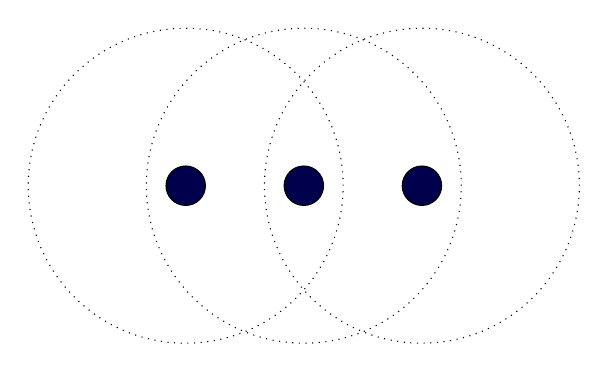
\begin{tikzpicture}
	\node at (0,0) [draw,circle,minimum width=4cm,dotted]{};
	\node at (0,0) [draw,circle,minimum width=.5cm,fill=blue!30!black]{};
	\node at (-1.5,0) [draw,circle,minimum width=4cm,dotted]{};
	\node at (-1.5,0) [draw,circle,minimum width=.5cm,fill=blue!30!black]{};
	\node at (1.5,0) [draw,circle,minimum width=4cm,dotted]{};
	\node at (1.5,0) [draw,circle,minimum width=.5cm,fill=blue!30!black]{};
	\end{tikzpicture}
}
\end{cf}

\begin{cf}{
	Why need link-layer ACK?\\
	Cannot detect all collision!
}
\end{cf}

\begin{cf}{
	\begin{tikzpicture}[scale=2]
		\draw[solid] (0,0) -- (0,3);
		\draw[solid] (2,0) -- (2,3);
	\end{tikzpicture}
	}
\end{cf}

\begin{cf}{
	\begin{tikzpicture}[scale=2]
		\draw[solid] (0,0) -- (0,3);
		\draw[solid] (1.5,0) -- (1.5,3);
		\draw[solid] (3,0) -- (3,3);
	\end{tikzpicture}
	}
\end{cf}

